\begin{figure}[h]
	\centering
	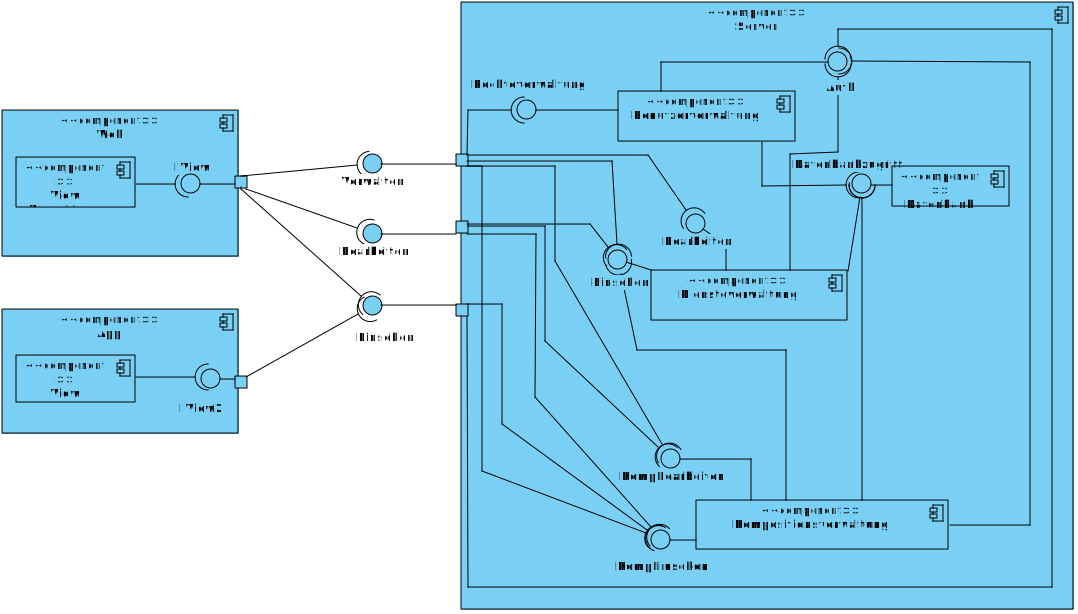
\includegraphics[width=\textwidth]{img/Diagramme/Komponenten}
	\caption{Komponentendiagramm}
	\label{fig:komponentendiagramm}
\end{figure}

\noindent
Die Serverkomponente bzw. das Backend beschreibt die internen Vorgänge der Software.
Diese Komponente ist über drei verschiedene Schnittstellen, welche die unterschiedlichen
Benutzerrechte repräsentieren, erreichbar.\\
In der Komponente ``Benutzerverwaltung'' werden die Daten der Benutzer aus der ``Datenbank'' ausgelesen und verarbeitet.
Dadurch kann die ``Benutzerverwaltung'' eine Authentifizierungsschnittstelle für die anderen Subkomponenten bereitstellen.
Zudem kann die Rechteverwaltung manipuliert werden, falls über die \textit{Verwalten}-Schnittstelle zugegriffen wird.
Die Komponente ``Diensteverwaltung'' liest die Daten der Dienste aus der ``Datenbank'' aus und verarbeitet diese.
Von außen kann auf die ``Diensteverwaltung'' durch die Schnittstellen \textit{Bearbeiten} und \textit{Einsehen} zugegriffen werden.
Die Schnittstelle \textit{Bearbeiten} ist nur für Administratoren über die Schnittstelle \textit{Verwalten} zugänglich.
Es werden bei jedem Zugriff die Rechte des zugreifenden Benutzers durch die Schnittstelle \textit{Auth} der ``Benutzerverwaltung'' überprüft.\\
Die Komponente ``Kompositionsverwaltung'' stellt die benötigten Funktionen für das Bearbeiten und Einsehen von Kompositionen zur Verfügung und bekommt die Daten dafür von den Komponenten ``Datenbank'' und ``Diensteverwaltung''.
Das Bearbeiten von Kompositionen ist nur über die Schnittstellen \textit{Bearbeiten} und \textit{Verwalten} möglich, das Einsehen auch über das \textit{Einsehen}-Interface.\\
Die Komponente ``Datenbank'' speichert alle nötigen Daten für die Komponenten ``Benutzer-'', ``Dienste-'' und ``Kompositionsverwaltung'' und stellt diese bei Bedarf zur Verfügung.
Zusätzlich kann man über die \textit{Einsehen}-Schnittstelle auch direkt auf die Authentifizierung zugreifen um eine initiale Registrierung und den Login zu ermöglichen.\\
\\
Die Komponente ``Web'' mit der Subkomponente ``View Verwaltung'' ist für die Darstellung in der Webapplikation zuständig.
Da man über die Weboberfläche verwalten, bearbeiten und einsehen können soll, ist die Web-Komponente auch mit all diesen Schnittstellen verbunden.\\
Die Komponente ``App'' mit der Subkomponente ``View'' dient zur Darstellung der angefragten Daten in der App.
In der App können nur Kompositionen eingesehen werden, daher ist diese nur mit der \textit{Einsehen}-Schnittstelle verbunden.
